\chapter{Fuel Cycle Sensitivity to Separation Efficiency}
\index{Fuel Cycle Sensitivity to Separation Efficiency@\emph{Fuel Cycle Sensitivity to Separation Efficiency}}
\label{ses_paper}



\section{Introduction}
\index{Introduction@\emph{Introduction}}
\label{ses_sec:intro}
As of 2008, the United States power reactor fleet has generated over
50,000 tonnes initial heavy metal (tIHM) of spent nuclear fuel (SNF). 
The quandary posed by this growing stockpile of SNF, combined with the
prospect of much larger inventories in the future, poses a considerable
obstacle to the development of nuclear energy.  While the technical
difficulty of storing and disposing of the SNF is considerable, it is
public trepidation that may have the strongest effect upon the future of
the industry.  

Partitioning and transmutation will significantly reduce the nuclear
waste disposal burden by recycling actinides from SNF in advanced
reactors and separating the most hazardous fission products for storage
in dedicated facilities or target irradiation.  Reprocessing technology
is one of the key components shared by all advanced fuel cycle concepts.
 Notably, the efficiency of the reprocessing facilities will have a
great impact on the performance of any advanced fuel cycle. 

This study investigates how the properties of the reprocessing facility,
in particular its separation efficiency for each of the partitioned
elements, affect the system characteristics of the fuel cycle. The
element-specific separation efficiency is defined as the mass ratio of
the recovered product to its input mass to the reprocessing facility. 
The fuel cycle system performance is characterized via three metrics:
fuel cycle cost, proliferation resistance and repository impact.  To
depict repository impact, the repository capacity is modeled as being
limited by thermal output; projected dose rate, mass inventory and waste
toxicity index are also quantified.  The study considers a single-tier
nuclear fuel cycle scenario in which light water reactors (LWRs) and 0.5
transuranic (TRU) conversion ratio (CR) sodium-cooled fast reactors are
deployed in an equilibrium that results in zero net TRU production. 
Actinide management schemes ranging from recycle of plutonium to full
TRU recycle are considered.

The objective of the work is to use essential physics models at multiple scales
to establish a technical basis for comparing the trade off between
repository footprint, system economics and proliferation resistance and
the performance characteristics of the reprocessing facilities.  This
work is significant because target separation efficiencies must be
identified at the earliest stages of reprocessing facility design.  The
models incorporate feedback between the separation efficiencies, reactor
performance and fuel cycle mass balances.  In that sense, this effort
expands upon work conducted under the auspices of the Global Nuclear
Energy Partnership \cite{repmodel} that addresses the correlation between heat load
and repository capacity.  Although there is not yet enough information
in the literature to correlate reprocessing costs to separation
efficiency, once such data is developed it can be coupled to this
framework, and the resulting tool would be an ideal platform for
selecting optimal separation efficiencies.

Section \ref{ses_sec:sys_modeling} of the paper describes the simulation and metric evaluation
methods used to study the selected fuel cycle scenarios.  In \S \ref{ses_sec:benchmarking}
the simulation approach is benchmarked against published results. 
Finally, \S \ref{ses_sec:conclusions} presents and discusses the results of the analyses.


\section{System Modeling Approach}
\index{System Modeling Approach@\emph{System Modeling Approach}}
\label{ses_sec:sys_modeling}
The closed fuel cycle selected for study includes uranium-fueled LWRs
as well as FR burners.  This fuel cycle was examined in great detail in 
\S \ref{1g_sec:FRFC}; a brief overview follows here.  After uranium oxide 
(UOX) fuel is discharged from the LWRs, it undergoes aqueous reprocessing 
to retrieve transuranics and fission products (FP).  A variety of UREX+ inspired
partitioning schemes are considered for this step; some or all of the
retrieved TRU elements are recycled into the FR TRU burner.  In
particular, Pu, Pu/Np, and full TRU recycle are studied.  FR spent fuel
is itself reprocessed and actinide species identified above are
recycled. Reprocessed burned uranium and depleted uranium are treated as
low level waste. Cs and Sr, as two strong heat contributors, are
reprocessed from SNF at an interim site before they decay to very low
level radioactive materials. The other FP will be sent to repository
with the residual TRU from reprocessing facility as high level waste
(HLW).  This scenario is equivalent to a case being considered by the
Global Nuclear Energy Partnership (GNEP) systems analysis group \cite{Piet2004}. 


\subsection{Overview of Methods}
\index{Overview of Methods@\emph{Overview of Methods}}
\label{ses_sec:method_overview}
The fuel cycle is specified by reactor material balances and material
flows between reactors and fuel cycle facilities.  Parameters related to
the LWR, for instance burnup and spent fuel isotopic composition, are
the reference values adopted in a recent OECD Nuclear Energy Agency
systems study \cite{NEA-5990}.  The fuel cycle material balance strategy for FR
multirecycle is identical to that used in both the OECD and the GNEP
studies: to reach the designated burnup level, the first core of the FR
is loaded with only the retrieved TRU and U from LWR SNF. The second and
subsequent cycle are loaded with TRU and U from FR SNF plus retrieved
top-up TRU from LWR SNF and depleted uranium (DU).  Cycles are continued
until the equilibrium state is reached.  It is important to dynamically
simulate the FR fuel composition at each pass, since critical system
variables such as partitioning strategy, cooling time and separation
efficiency exert a strong effect on the reactor physical characteristics
of subsequent recycle passes. 

Therefore, a dynamic fast reactor simulation tool is developed to
simulate this process and calculate the isotopic composition of the FR
fuel at each pass.  This model is composed of three components: burnup,
reactivity and decay.  The reactivity module returns the fresh fuel
composition for a specified discharge burnup given the number of batches
in the fuel management scheme, while the burnup module calculates the
isotopic composition of the burned fuel for a specified fresh fuel
composition and discharge burnup target.  The decay model applies the
Bateman equations to a mass of fuel and returns the isotopic output
after a given decay time.  

After the fuel isotopic compositions at each pass are determined, the
inventory at each stage can be calculated and the system performance of
the fuel cycle evaluated.  System performance is characterized through
fuel cycle cost, proliferation resistance and repository impact. 
Repository impact is represented by both repository capacity limited by
thermal constraints and the projected dose rate from a fully loaded
repository.  



\subsection{System Performance Assessment}
\index{System Performance Assessment@\emph{System Performance Assessment}}
\label{ses_sec:spa}
A number of metrics are applied to the material balances to translate
them into decision-relevant information.  These metrics include the fuel
cycle cost, proliferation resistance, repository capacity via thermal
limits, dose release and toxicity.

The fuel cycle cost is the cost to buy the fresh fuel to be loaded into
the reactors and the cost for recycling and waste disposal.  Its
components include U ore purchase, U conversion, U enrichment, LWR fuel
fabrication, FR fuel fabrication, SNF storage, SNF reprocessing, LLW
(Low Level Waste) disposal, LLW-GTCC (Greater than Class C) disposal,
HLW (High Level Waste) disposal. The unit costs for these components are
collected from published literature as described in Section 3. 

Procedures for calculating the FCC were presented in \S \ref{1g_paper} and the
method used in this study will be summarized only briefly.  The FCC\subscript{t}
total charge is the sum of charges for all components of the fuel cycle
cost.  It is calculated using the formulation
\begin{equation}
\label{ses_FCC}
\mbox{FCC}_t = C_u \cdot s
\end{equation}
where $C_u$ [\$/KgHM or \$/SWU] is the unit charge and $s$ [kgHM/yr or SWU/yr] 
is the service ammount. The FCC [\$/MWh] may then be obtained by dividing the 
FCC\subscript{t} total charge [\$/yr] by the annual electricity production [MWh/yr].

A fuzzy logic based barrier method is used to evaluate the
proliferation resistance of the fuel cycle system \cite{Li2009}. The proliferation
resistance is defined here as the ability of the system to intrinsically
protect itself against proliferators seeking to construct a nuclear
explosive device. The method relies upon a group of system-dependent,
measurable or quantifiable variables to define proliferation barrier
effectiveness of a system as fuzzy numbers. 
Table \ref{ses_table1} lists the important variables required for
the evaluation. Information at each stage of the fuel cycle system are
collected and processed for the proliferation resistance evaluation.
Table \ref{ses_table2} shows the stages involved in the fuel cycle system, type and
inventory of materials handled in the stage.


\begin{table}[htbp]
\begin{center}
\caption{Required Inputs for PR Evaluation}
\label{ses_table1}
\begin{tabular}{|l|l|c|l|}
\hline
\textbf{Item} & \textbf{Name} & \textbf{Unit} & \textbf{Comments} \\
\hline
1  & StageWeight     &             & Concentration of sensitive materials\\
2  & CriticalMass    & kg          & Bare sphere Critical Mass (CM)\\
3  & Enrichment      & \%          & Equivalent Enrichment (\nuc{U}{233}, \nuc{U}{235}, \nuc{Pu}{239})\\
4  & SFN             & n/s/kg      & Spontaneous neutron generation rate\\
5  & HeatRate        & W/kg        & Heat generation rate\\
6  & Radiation       & MeV/s/kg    & Gamma Radiation\\
7  & SeparationCost  & \$/kg       & Cost to extract the fissile materials\\
8  & DoseRate        & mrem/hr/kg  & Dose rate at 1-meter distance\\
9  & Concentration   & \# of CM/kg & Concentration of fissile material\\
10 & Detectability   &             & Detectability levels (Five levels)\\
11 & FacilityModTime & weeks       & Modification timeto produce 1 CM in a year\\
12 & AccessFrequency & days/yr     & Frequency of possible access to facility\\
13 & AvailableMass   & \# of CM    & Available fissile materials\\
14 & MeasureUncert   & \# of CM/yr & Uncertainty of measurement\\
15 & Knowledge       & yr          & Time to apply skills to weapons programs\\
16 & Time            & yr          & Residence time of the materials \\
\hline
\end{tabular}
\end{center}
\end{table}


\begin{table}[htbp]
\begin{center}
\caption{System Material Characteristics}
\label{ses_table2}
\begin{tabular}{|l|l|l|}
\hline
\textbf{Stage \#} & \textbf{Description} & \textbf{Material Form} \\
\hline
1  & U Ore & U\subscript{3}O\subscript{8} \\
2  & U Conversion         & UF\subscript{6}\\
3  & U Enrichment         & UF\subscript{6} (Enriched)\\
4  & LWR Fuel Fabrication & UOX\\
5  & FR Fuel Fabrication  & IMF\\
6  & LWR                  & UOX\\
7  & FR                   & IMF\\
8  & Reprocessing         & TRU\\
9  & SNF Storage          & SNF (UOX \& IMF)\\
10 & LLW Disposal         & BU DU\\
11 & LLW GTCC Disposal    & CS/SR\\
12 & HLW/TRU Disposal     & FP, Residual TRU\\
\hline
\end{tabular}
\end{center}
\end{table}


The repository impact is quantified through capacity limitations imposed
by thermal constraints as well as the dose release from a fully loaded
repository. The Yucca Mountain repository with footprint 1165.8 acres is
used for this study \cite{Wiegland2006}.	

The repository capacity is constrained by the thermal limits placed on
the rocks to ensure the successful performance of the engineering
barrier system employed in the repository. The thermal restraints
considered in this study are $200^\circ$ C on drift walls and
$96^\circ$ C midway between drifts. The repository capacity is
estimated using both a simplified repository thermal analysis SRTA tool
and mass based prediction model.  The SRTA is a code based on analytical
solution of models of the Yucca Mountain repository \cite{Li2010a}. The code
calculates the temperature of give location in the repository and this
function is used to determine the repository capacity. 

To evaluate the dose release rate for a loaded repository, a simplified
performance assessment tool is used in this study. This model has
four main parts: source term model, unsaturated zone transport model,
saturated zone transport model, and dose analysis model. The transport
in the saturated zone was modeled based on a 2D analytic solution to the
advection dispersion equation for contaminants. Human exposure to
radionuclides was assumed to occur only through the drinking of
contaminated groundwater from a well in a single location.




\section{Benchmarking}
\index{Benchmarking@\emph{Benchmarking}}
\label{ses_sec:benchmarking}
The OECD Nuclear Energy Agency has gathered participants from several
countries to perform system evaluation of several advanced fuel cycle
designs \cite{NEA-5990}. In this study, the advanced fuel cycles are compared
with the reference once-through thermal reactor system.


\subsection{Benchmark Cases}
\index{Benchmark Cases@\emph{Benchmark Cases}}
\label{ses_sec:benchmark_cases}
The system simulation tool developed in this study is applied to the two
scenarios defined in the NEA study for benchmark. The scenarios are
notated ``scheme 1a'' and ``scheme 3a''.  Scheme 1a is a once-through
PWR system.  Enriched uranium (4.9\% U235) is burned in a PWR to 60
GWd/MTHM.  The SNF is sent to a storage facility for 7 year decay.
Another 50 years cooling is assumed before the SNF is disposed in the
repository.  The key fuel cycle parameters describing this case are
presented in Table \ref{ses_table3}.

\begin{table}[htbp]
\begin{center}
\caption{Scheme 1a System and Reactor Design: 0.71\% Natural U is enriched 
to 4.90\% for UOX with tail enrichment 0.25\%; Designed capacity of the PWR 
is 1450 MWe. The load factor is 90\%. The burnup is 60 MWd/kgIHM.}
\label{ses_table3}
\begin{tabular}{|l|c|}
\hline
\textbf{Stage \#} & \textbf{Description} \\
\hline
\multicolumn{2}{|c|}{Mass Flows for Scheme 1a (kgIHM/TWh\subscript{e})}\\
\hline
Natural U  & 20723\\
Depleted U & 18673\\
UOX        & 2050\\
\hline
\multicolumn{2}{|c|}{Element in SNF after 7 yrs decay}\\
\hline
U  & 1890\\
Pu & 26\\
Np & 1.9\\
Am & 1.6\\
Cm & 0.28\\
FP & 130\\
\hline
\end{tabular}
\end{center}
\end{table}



Scheme 3a is a closed fuel cycle design using a fast reactor burner to
consume recycled TRU from the PWR SNF.  The precise isotopic composition
of this fuel was not provided in the study; therefore ORIGEN was used to
calculate it.  The results, which act as an input to the FR burnup
calculations, are given in Table \ref{ses_table4}.  For this calculation, as stipulated
in the OECD study, the uranium was enriched to 4.2\% U-235 and burned in
the PWR to 50 MWd/kgIHM (megawatt-days per kilogram initial heavy metal). 

\begin{table}[htbp]
\begin{center}
\caption{Nuclide Composition [kg\subscript{i}/kgIHM] of LWR TRU feed to FR after 6 yr Cooling}
\label{ses_table4}
\begin{tabular}{|l|c|c|}
\hline
\textbf{Nuclide} & \textbf{PWR Fresh} & \textbf{PWR SNF} \\
\hline
\nuc{Am}{241}    &                    & 4.74E-04\\
\nuc{Am}{243}    &                    & 2.13E-04\\
\nuc{Cm}{242}    &                    & 3.80E-09\\
\nuc{Cm}{243}    &                    & 6.97E-07\\
\nuc{Cm}{244}    &                    & 7.21E-05\\
\nuc{Cm}{245}    &                    & 4.38E-06\\
\nuc{Cm}{246}    &                    & 6.91E-07\\
\nuc{Cm}{247}    &                    & 9.03E-09\\
\nuc{Cm}{248}    &                    & 6.36E-10\\
\nuc{Np}{237}    &                    & 7.62E-04\\
\nuc{Pu}{238}    &                    & 2.95E-04\\
\nuc{Pu}{239}    &                    & 5.89E-03\\
\nuc{Pu}{240}    &                    & 2.73E-03\\
\nuc{Pu}{241}    &                    & 1.31E-03\\
\nuc{Pu}{242}    &                    & 8.59E-04\\
\nuc{U}{234}     &                    & 1.64E-05\\
\nuc{U}{235}     & 4.20E-02           & 6.83E-03\\
\nuc{U}{236}     &                    & 5.65E-03\\
\nuc{U}{238}     & 9.58E-01           & 9.23E-01\\
\hline
\end{tabular}
\end{center}
\end{table}


The retrieved Pu and other MA are used for fast reactor fresh fuel. The
TRU in the 3 years decayed fast reactor spent fuel is fully reprocessed
and recycled into the fast reactor. The fission products and actinides
lost in reprocessing are sent to repository as high level waste after 50
years cooling.  The load factor is 90\% for PWRs and 85\% for FRs.  In
this benchmark scenario, the separation efficiency for all species is
99.9\%.  The top-level system parameters for Scheme 3a are presented in
Table \ref{ses_table5}.

\begin{table}[htbp]
\begin{center}
\caption{Scheme 3a System and Reactor Design:
0.71\% natural U is enriched to 4.20\% for UOX with tail enrichment
0.25\%; capacity of the PWR is 1450 MWe. The load factor is 90\%. The
burnup is 50 GWd/tIHM for PWR and the spent fuel is decayed for 6 yrs
before it is reprocessed. The retrieved TRU is mixed with depleted U for
FR fresh fuel. The burnup for FR is 140 GWd/tIHM and the FR spent fuel
is reprocessed after 3 yrs decay. Capacity of the FR is 600 MWe and the
load factor is 85\%. 36.8\% of fleet electricity comes from FR.}
\label{ses_table5}
\begin{tabular}{|l|c|}
\hline
\textbf{Stage \#} & \textbf{Description} \\
\hline
\multicolumn{2}{|c|}{Mass Flows for Scheme 3a (kgIHM/TWh\subscript{e})}\\
\hline
Natural U & 12991\\
UOX       & 1513\\
FR FF     & 289\\
\hline
\multicolumn{2}{|c|}{Element in HLW after Separation} \\
\hline
U  & 1.588\\
Pu & 0.084\\
Np & 0.0027\\
Am & 0.006\\
Cm & 0.0026\\
FP & 117.5\\
\hline
\end{tabular}
\end{center}
\end{table}


The unit costs used are summarized in Table 6. The disposal costs for
HLW and SNF are calculated from the information available in an earlier
OECD NEA report ().  This report recommends 210,000 \$/m3 and 400,000
\$/m3 for the disposal charges of SNF and HLW respectively. After
conditioning, 1 tIHM SNF will result in 2 m\superscript{3} waste, i.e., 420 \$/kgIHM.
For vitrified HLW, a canister of volume 0.18 m3 is taken to contain 47.6
kg fission products and 3.55 kg actinides.  Therefore the disposal
charge for HLW becomes 1408 \$/kgIHM.

\begin{table}[htbp]
\begin{center}
\caption{Unit Costs used in Benchmark Study}
\label{ses_table6}
\begin{tabular}{|l|c|c|}
\hline
\textbf{Item}                   & \textbf{Unit} & \textbf{Value} \\
\hline
U Ore (yellow cake)             & \$/kgHM       & 50.0 \\
U Conversion                    & \$/kgHM       & 5.0 \\
U Enrichment                    & \$/SWU        & 100.0 \\
LWR Fuel Fabrication            & \$/kgHM       & 250.0 \\
FR Fuel Fabrication             & \$/kgHM       & 2600.0 \\
Reprocessing for LWR Spent Fuel & \$/kgHM       & 800.0 \\
Reprocessing for FR Spent Fuel  & \$/kgHM       & 2500.0 \\
SNF Storage                     & \$/kgHM       & 90.0 \\
LLW Near Surface Disposal       & \$/kgHM       & 3.60 \\
LLW GTCC Disposal               & \$/kgHM       & 381.0 \\
SF Disposal                     & \$/kgHM       & 420.0 \\
HLW Disposal                    & \$/kgHM       & 1408.0 \\
\hline
\end{tabular}
\end{center}
\end{table}



\subsection{Benchmark Results}
\index{Benchmark Results@\emph{Benchmark Results}}
\label{ses_sec:benchmark_results}
The composition of FR fuel at equilibrium is calculated with the
dynamic FR simulation tool described in Section 2.2\ref{} and compared to
results published in the OECD study.  The fuel cycle cost is also
benchmarked using the unit costs shown in Table 6 and methodology
depicted in Section 2.3.  The inventory and FCC comparisons are shown in
Table \ref{ses_table7} for both schemes.  As mentioned above, ORIGEN was used to
compute the PWR material balance.

The inventories of major actinides in the HLW in scheme 1a from both
studies are in close agreement with relative errors of less than 10\%,
except Cm which has a smaller absolute inventory in the system. The mean
value of FCC from OECD study is approximately 4.7 \$/MWh for scheme 1a
from the sensitivity result in the OECD report. The value of 4.27 \$/MWh
in this study results less than 10\% error.  This variation stems from
minor differences in the cost assessment methodology and back-end unit
costs. 

Scheme 1a does not benchmark the dynamic FR simulation tool; however it
does provide the TRU isotopics that serve as the starting point for the
calculations carried out by the tool.  The procedure described in
Section 2.2 was used to perform cycle iterations until the FR fuel
composition converged to equilibrium.  Good agreement on the PWR to FR
power split, charge and discharge inventories and the FCC for scheme 3a
can be observed.  Whether the difference observed for scheme 3a can be
ascribed to the FR simulation tool, or to inconsistencies in the LWR
feed arising from the absence of isotopic data in the OECD study, cannot
be established.  However in view of the great complexity of the fuel
cycle system the agreement is strong.  For instance, the design
parameters of the FR were not given in sufficient detail to perform
transport-burnup calculations, so a case-specific cross section library
could not be prepared and available data for a FR that shares many
properties of the OECD study reactor (e.g., sodium-cooled, metallic
fuel, similar pitch and fuel pin radius) were used instead.

\begin{table}[htbp]
\begin{center}
\caption{Scheme 1a Benchmark Results}
\label{ses_table7}
\begin{tabular}{|l|c|c|c|}
\hline
\textbf{Parameter} & \textbf{OECD 2006} & \textbf{Results} & \textbf{\% Differnec} \\
\hline
UOX FF [kg/TWh\subscript{e}]    & 2050  & 2050    & 0.0 \\
U Natural [kg/TWh\subscript{e}] & 20723 & 20722.8 & 0.0 \\
U in HLW [kg/TWh\subscript{e}]  & 1890  & 1896    & 0.3 \\
Pu in HLW [kg/TWh\subscript{e}] & 26    & 24      & -8.86 \\
Np in HLW [kg/TWh\subscript{e}] & 1.9   & 2.0     & 4.29 \\
Am in HLW [kg/TWh\subscript{e}] & 1.6   & 1.7     & 8.55 \\
Cm in HLW [kg/TWh\subscript{e}] & 0.28  & 0.24    & -15.17 \\
FP in HLW [kg/TWh\subscript{e}] & 130   & 127     & -2.61 \\
FCC [\$/MWh]                    & 4.7   & 4.27    & -9.15 \\
\hline
\end{tabular}
\end{center}
\end{table}


\begin{table}[htbp]
\begin{center}
\caption{Scheme 3a Benchmark Results}
\label{ses_table7_3a}
\begin{tabular}{|l|c|c|c|}
\hline
\textbf{Parameter} & \textbf{OECD 2006} & \textbf{Results} & \textbf{\% Differnec} \\
\hline
Electricity Share: PWR [\%]     & 63.2   & 66.1    & 4.59 \\
Electricity Share: FR [\% ]     & 36.8   & 33.9    & -7.88 \\
UOX FF [kg/TWh\subscript{e}]    & 1513   & 1583    & 4.63 \\
U Natural [kg/TWh\subscript{e}] & 12991  & 13593.2 & 4.64 \\
UOX FF [kg/TWh\subscript{e}]    & 289    & 266.2   & -7.88 \\
U in HLW [kg/TWh\subscript{e}]  & 1.588  & 1.6361  & 3.03 \\
Pu in HLW [kg/TWh\subscript{e}] & 0.084  & 0.0814  & -3.10 \\
Np in HLW [kg/TWh\subscript{e}] & 0.0027 & 0.0030  & 10.52 \\
Am in HLW [kg/TWh\subscript{e}] & 0.006  & 0.0073  & 21.62 \\
Cm in HLW [kg/TWh\subscript{e}] & 0.0026 & 0.0020  & -21.8 \\
FP in HLW [kg/TWh\subscript{e}] & 117.5  & 119.3   & 1.59 \\
FCC [\$/MWh]                    & 5.5    & 5.13    & -6.73 \\
\hline
\end{tabular}
\end{center}
\end{table}


The OECD group has also conducted repository performance studies for
their schemes 1a and 3c, where 3c is a FR only closed fuel cycle.
Because the HLW from both scheme 3c and 3a is mainly composed of FP, the
repository performance assessments for schemes 3a and 3c can be expected
to yield nearly equivalent results. 

The energy that has been produced by disposed waste in a fully loaded
salt-based repository is given as 6615 TWh for scheme 1a and 26930 TWh
for scheme 3c.  In other words, the waste from closed fuel cycle 3c
would have generate 4.0 times as much electricity as scheme 1a waste
placed in the same repository.  Using the repository capacity assessment
methodology described in Section 2.3 \ref{}, the energy that has been produced
by disposed waste in a tuff-based repository in this study is 28286 TWh
for scheme 1a and 186365.3 TWh for scheme 3a. Therefore, the current
work predicts that scheme 3a can, when compared to scheme 1a, generate
6.6 times as much electricity given a repository of specified thermal
capacity. This is higher than the 4.0 ratio calculated in the OECD
study, but the difference in the geologic medium -- salt versus tuff --
complicates the comparison.



\section{Case Study and Results}
\index{Case Study and Results@\emph{Case Study and Results}}
\label{ses_sec:case_study}
For the study of system sensitivity to separation efficiency and
partitioning strategy, we consider a fleet in which PWRs and CR 0.5 FRs
are in equilibrium.  This is the same concept as was put into practice
in scheme 3a of the OECD study.


\subsection{Definition of the Cases}
\index{Definition of the Cases@\emph{Definition of the Cases}}
\label{ses_sec:case_def}
The present-day industrial scale reprocessing technology, PUREX,
retrieves U and Pu from SNF. Fuel cycle strategies developed under the
DOE Advanced Fuel Cycle Initiative called for extraction of Np with Pu
to ease proliferation concerns, material accountability and tracking
procedures for the product stream. It has been convincingly established
(see for instance (  NOTEREF 
MERGEFORMAT  2 )) that separation of Am and Cm as well is necessary to
maximize the benefit of increasing the capacity of a repository that is
constrained by thermal limits.  The repository capacity can be further
expanded by removing Cs and Sr for interim storage. Therefore, in this
study, four partitioning strategies are compared:

\begin{itemize}
    \item Stra1: Separation of U and Pu to be reused in FR
    \item Stra2: Separation of U, Np and Pu to be reused in FR
    \item Stra3: Separation of U, Np, Pu, Am and Cm to be reused in FR
    \item Stra4: Separation of U, Np, Pu, Am and Cm to be reused in FR, and
          separation of Cs and Sr for interim storage
\end{itemize}

In a scenario involving multi-recycle of spent fuel, the cumulative
effect of reprocessing losses at each recycle can become quite
significant, so that only with high separation efficiencies can the full
benefit of the multi-recycle strategy be realized.  For example, the NEA
study indicated that for their cases 3a and 3c less than 0.01\% loss is
needed to reach a factor of 100 reduction in the high level waste heat
burden to the repository.  Therefore, to develop an understanding of the
sensitivity of the system performance metrics to separation efficiency,
four levels are studied:

\begin{itemize}
    \item Level1: 90\%
    \item Level2: 99\% 
    \item Level3: 99.9\%
    \item Level4: 99.99\%
\end{itemize}

The separation efficiencies of all elements are assumed to be the same.
There is no \emph{a priori} reason to make this assumption as no aspect of
reprocessing facility design or operation imposes such a constraint. 
Instead, this assumption was made to simplify the analysis and prevent
an egregious proliferation of cases to be studied.  In addition, and for
similar reasons of clarity, the aqueous PWR fuel reprocessing and the
electrochemical FR metallic fuel separations share the same
efficiencies. Four partitioning strategies and four separation
efficiency levels generate the 16 cases defined in Table \ref{ses_table8}.  
Table \ref{ses_table9} shows the elemental separation efficiencies for the cases; an entry of
zero indicates that the element remains with the repository-bound waste
stream.

\begin{table}[htbp]
\begin{center}
\caption{16 Case Definitions}
\label{ses_table8}
\begin{tabular}{|l|c|c|c|c|}
\hline
                & \textbf{Stra1} & \textbf{Stra2} & \textbf{Stra3} & \textbf{Stra4} \\
\hline
\textbf{Level1} & Case01         & Case02         & Case03         & Case04 \\
\textbf{Level2} & Case1          & Case2          & Case3          & Case4 \\
\textbf{Level3} & Case11         & Case12         & Case13         & Case14 \\
\textbf{Level4} & Case21         & Case22         & Case23         & Case24 \\
\hline
\end{tabular}
\end{center}
\end{table}

\begin{table}[htbp]
\begin{center}
\caption{Separation Efficiencies by Case and Element}
\label{ses_table8}
\begin{tabular}{|l|c|c|c|c|c|c|c|}
\hline
\textbf{Case} & \textbf{U} & \textbf{Np} & \textbf{Pu} & \textbf{Am} & \textbf{Cm} & \textbf{Cs} & \textbf{Sr} \\
case01 & 0.9    & 0      & 0.9    & 0      & 0      & 0      & 0      \\
case02 & 0.9    & 0.9    & 0.9    & 0      & 0      & 0      & 0      \\
case03 & 0.9    & 0.9    & 0.9    & 0.9    & 0.9    & 0      & 0      \\
case04 & 0.9    & 0.9    & 0.9    & 0.9    & 0.9    & 0.9    & 0.9    \\
case1  & 0.99   & 0      & 0.99   & 0      & 0      & 0      & 0      \\
case2  & 0.99   & 0.99   & 0.99   & 0      & 0      & 0      & 0      \\
case3  & 0.99   & 0.99   & 0.99   & 0.99   & 0.99   & 0      & 0      \\
case4  & 0.99   & 0.99   & 0.99   & 0.99   & 0.99   &0.99    & 0.99   \\
case11 & 0.999  & 0      & 0.999  & 0      & 0      & 0      & 0      \\
case12 & 0.999  & 0.999  & 0.999  & 0      & 0      & 0      & 0      \\
case13 & 0.999  & 0.999  & 0.999  & 0.999  & 0.999  & 0      & 0      \\
case14 & 0.999  & 0.999  & 0.999  & 0.999  & 0.999  & 0.999  & 0.999  \\
case21 & 0.9999 & 0      & 0.9999 & 0      & 0      & 0      & 0      \\
case22 & 0.9999 & 0.9999 & 0.9999 & 0      & 0      & 0      & 0      \\
case23 & 0.9999 & 0.9999 & 0.9999 & 0.9999 & 0.9999 & 0      & 0      \\
case24 & 0.9999 & 0.9999 & 0.9999 & 0.9999 & 0.9999 & 0.9999 & 0.9999 \\
\hline
\end{tabular}
\end{center}
\end{table}



\subsection{Results and Discussion}
\index{Results and Discussion@\emph{Results and Discussion}}
\label{ses_sec:res_disc}
The 16 cases defined in previous chapter have each been modeled through
the transient phase to equilibrium with the FR material balance tool
described in Section 2.2.  In addition, the performance metrics defined
in Section 2.3 have been calculated.  Table \ref{ses_table_10} lists the fraction of
equilibrium reactor fleet electrical power generated by the FRs.  Note
that for neutronic purposes Stra3 is the same as Stra4 in which Cs and
Sr are partitioned.  For each strategy, higher separation efficiency
leads to higher FR share because more TRU are reused from LWR SNF and FR
SNF.  

\begin{table}[htbp]
\begin{center}
\caption{FR Share of Fleet Electricity Generation [\%]}
\label{ses_table10}
\begin{tabular}{|l|c|c|c|c|}
\hline
                & \textbf{Stra1} & \textbf{Stra2} & \textbf{Stra3} & \textbf{Stra4} \\
\hline
\textbf{Level1} & 26.0           & 26.0           & 25.6           & 25.6 \\
\textbf{Level2} & 33.0           & 33.0           & 33.0           & 33.0 \\
\textbf{Level3} & 33.8           & 33.8           & 33.9           & 33.9 \\
\textbf{Level4} & 33.9           & 33.9           & 34.0           & 34.0 \\
\hline
\end{tabular}
\end{center}
\end{table}

The system performance of the fuel cycle for the 16 cases will be
discussed separately for material balance and isotopics, FCC,
proliferation resistance and repository performance.


\subsubsection{Material Balance and Isotopics}
\index{Material Balance and Isotopics@\emph{Material Balance and Isotopics}}
\label{ses_sec:mat_balance}
Table \ref{ses_table11} displays the parameters input to the FR material balance tool.
Note that the partitioning strategies and separation efficiencies are
also vital inputs to the model.  FR operations are simulated until
equilibrium is attained.

\begin{table}[htbp]
\begin{center}
\caption{Input Parameters to FR Material Balance Model}
\label{ses_table11}
\begin{tabular}{|l|c|}
\hline
\textbf{Parameter} & \textbf{Value} \\
\hline
FR Discharge Burnup (BUd)             & 140 MWd/kg \\
Number of FR Fuel Batches	          & 3 \\
FR Non-Leakage Probability ($P_{NL}$) & 0.65\\
Cross Section Library                 & \S \ref{1g_paper} \\
Isotopes to Converge for Equilibrium  & \nuc{Pu}{239}, \nuc{Pu}{240}, \nuc{Pu}{242} \\
Post-discharge Cooling Time           & 3 years\\
\hline
\end{tabular}
\end{center}
\end{table}



Figure \ref{ses_fig06} shows the mass fraction [kg/kgIHM] of each of the four
input streams, DU, LWR-TRU, FR-U and FR-TRU, to FR fuel fabrication as a
function of FR recycle number.  Self recycle of FR SNF begins on pass 2.

It can be seen that the top-up drawn from the recycled LWR fuel is
predominantly LWR-TRU, but the gross mass fraction of each of the four
streams converges quickly toward an apparent equilibrium after only a
few cycles.  The criterion described in Table \ref{ses_table11} leads to equilibrium
being reached at cycle 10.

\begin{figure}[htbp]
\caption{Input Streams to FR Fuel Fabrication [kg/kgIHM]}
\label{ses_fig06}
\begin{center}
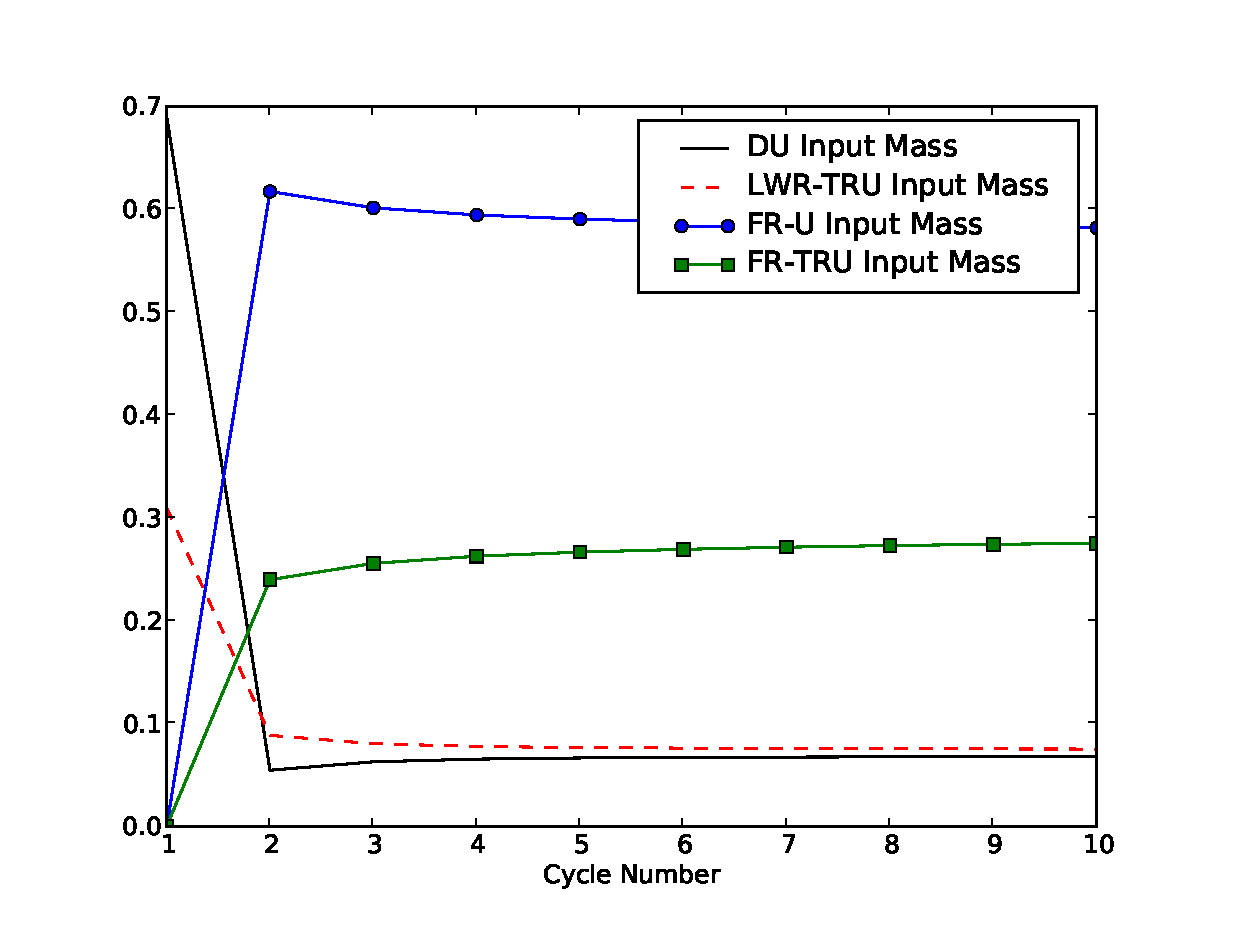
\includegraphics[scale=0.5]{se_sensitivity/figs/MassStreams.eps}
\end{center}
\end{figure}


The fast reactor output stream is a function of cycle number. 
Individual isotopes contained in the FR fuel do not necessarily converge
after only a handful of cycles.  Figure \ref{ses_fig07} shows the mass fractions at
discharge of \nuc{Np}{237}, \nuc{Pu}{239}, \nuc{Am}{241} and \nuc{Cm}{244}.  
It can be seen that the higher A number actinides have not yet converged even after 10 cycles. 
Also noteworthy is the dependence of the isotopic composition of the FR
fuel upon separation efficiency.  The higher A number species are
especially strongly affected by the efficiency, with the \nuc{Cm}{244}
inventory, for example, differing by 20\% at equilibrium for the 90\%
efficiency case versus the 99.99\% case.  Fig. 8 plots the fraction of
uranium and transuranics relative to the total actinide content of the
output stream.

\begin{figure}[htbp]
\caption{Input and Output Mass [kg/kgIHM] for Selected Actinides at Two Separation Efficiencies}
\label{ses_fig07}
\begin{center}
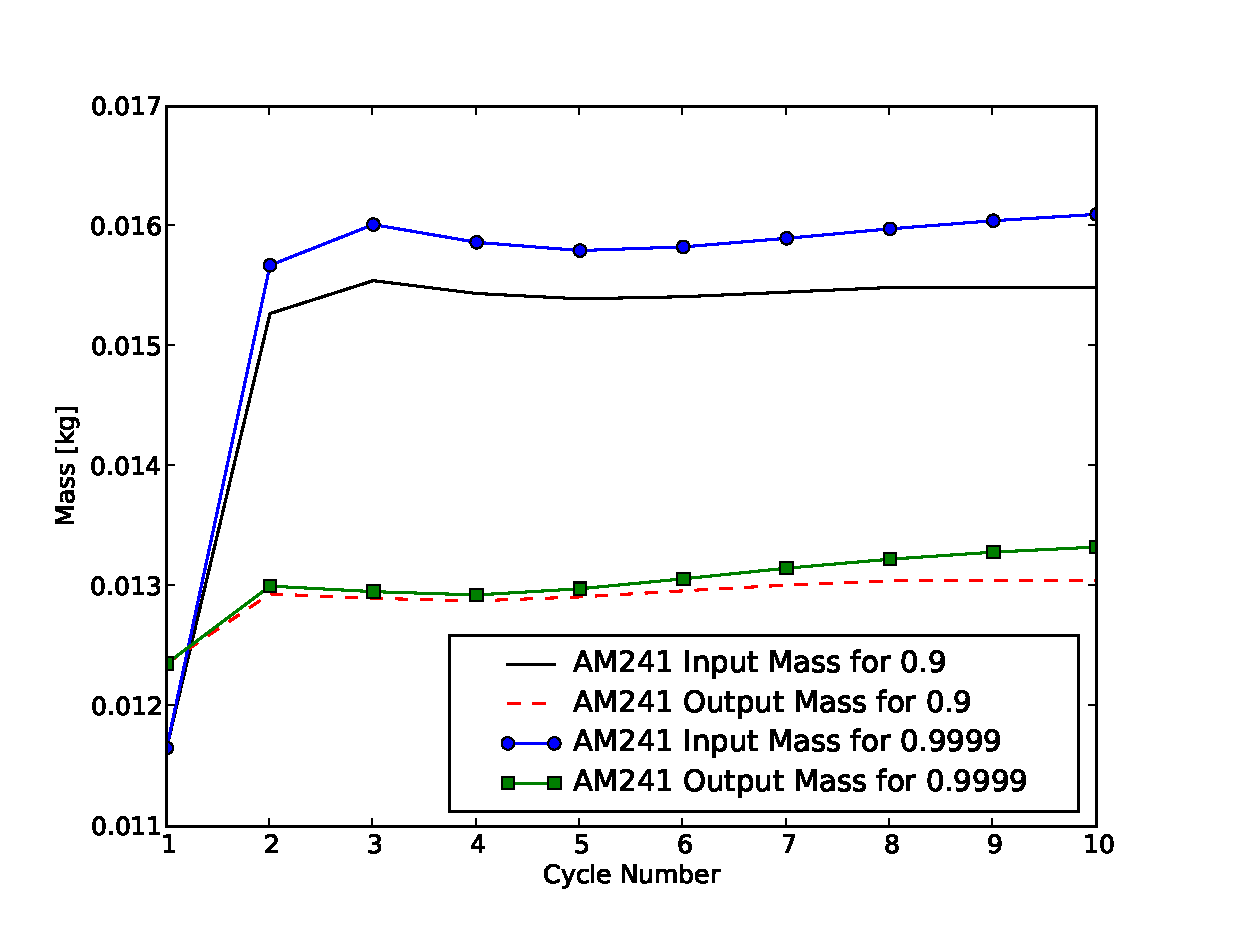
\includegraphics[scale=0.3]{se_sensitivity/figs/AM241InOutSepEff.eps}
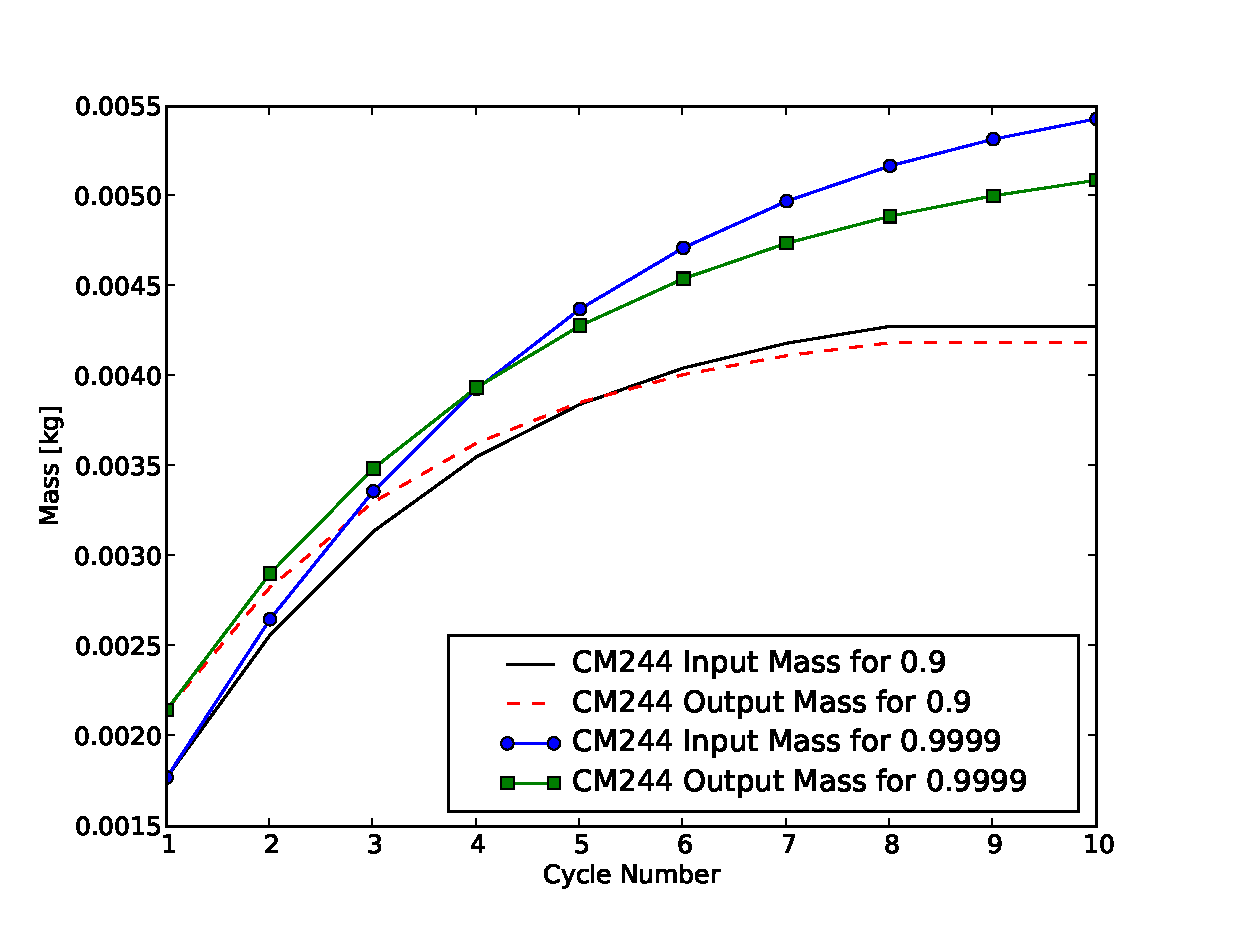
\includegraphics[scale=0.3]{se_sensitivity/figs/CM244InOutSepEff.eps}
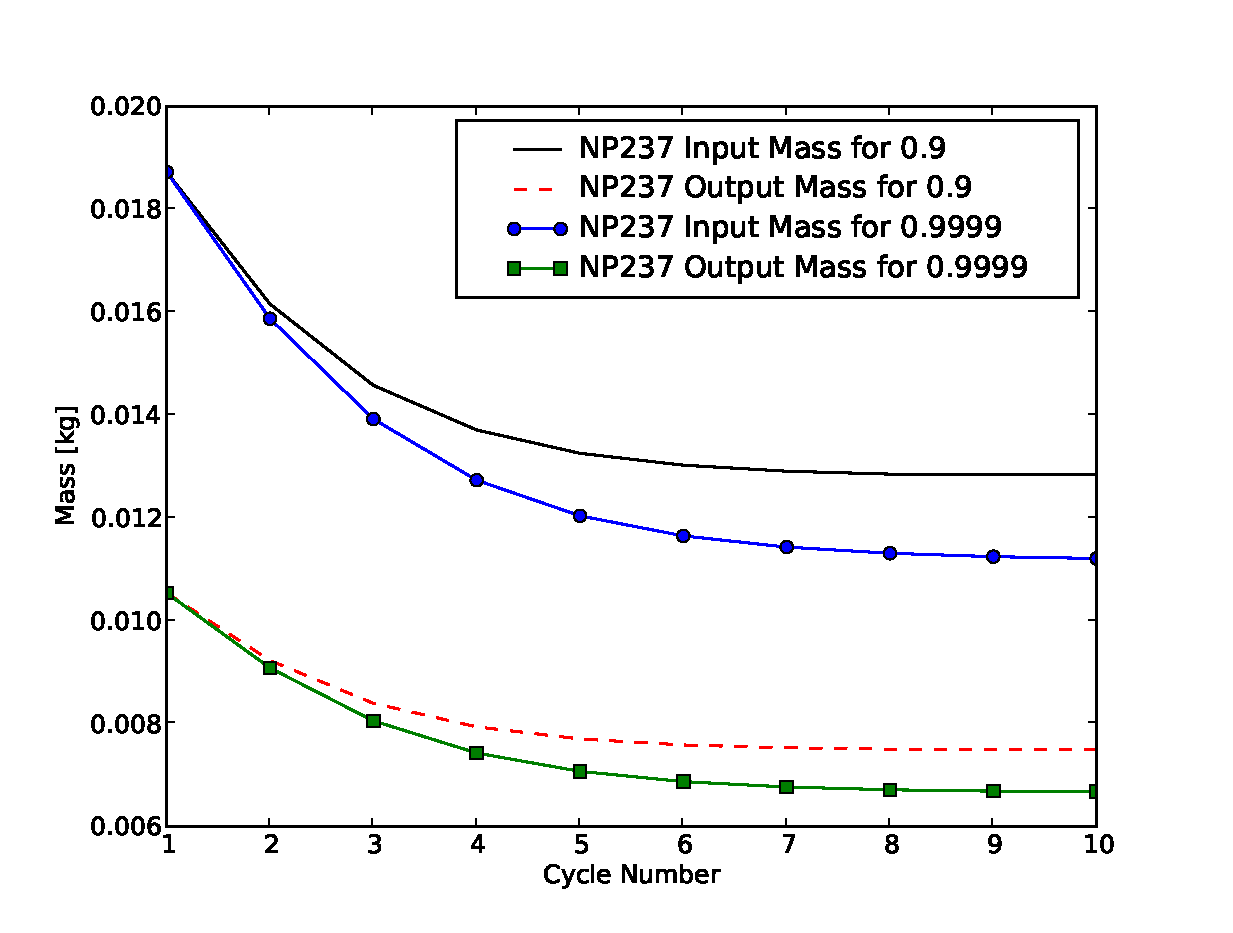
\includegraphics[scale=0.3]{se_sensitivity/figs/NP237InOutSepEff.eps}
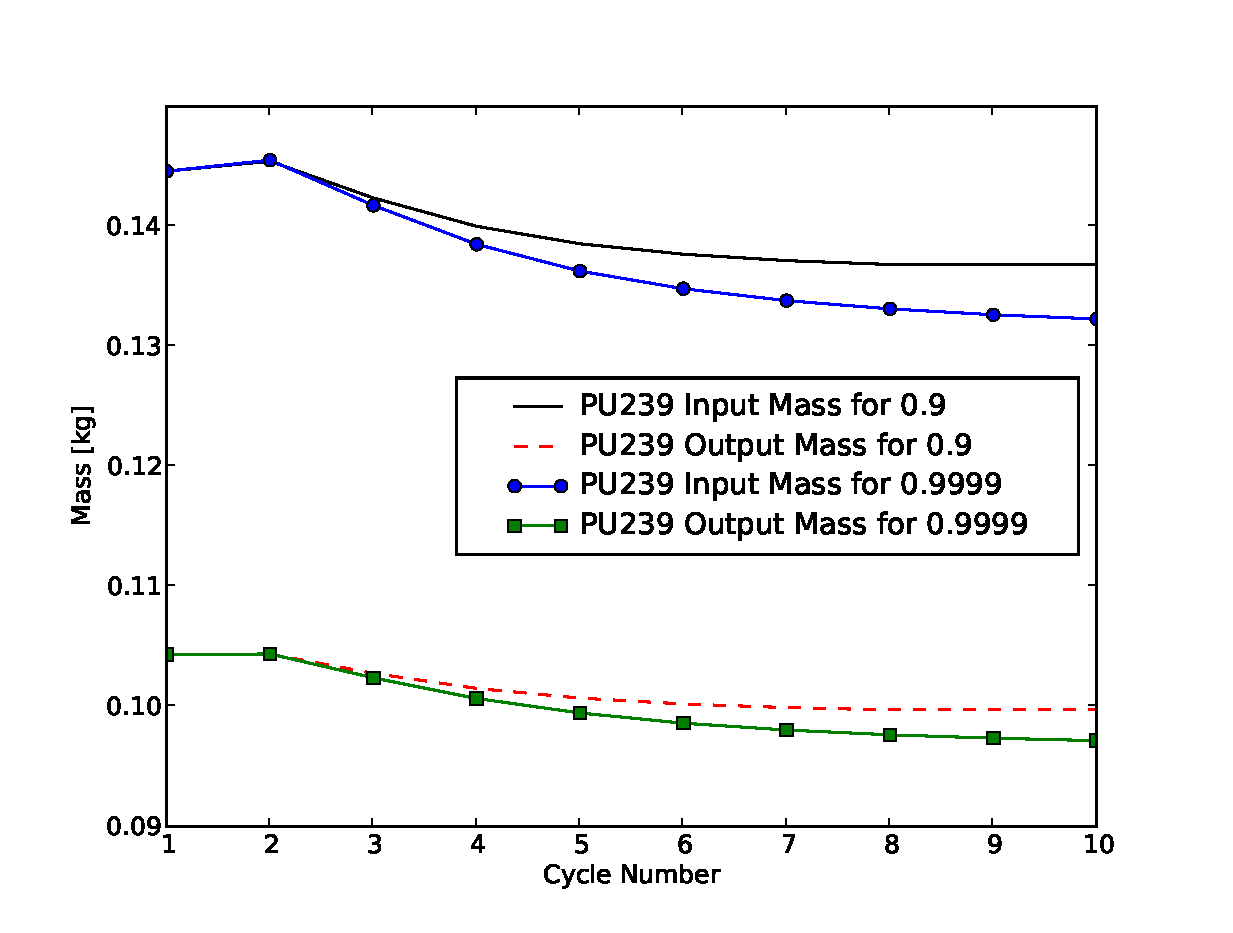
\includegraphics[scale=0.3]{se_sensitivity/figs/PU239InOutSepEff.eps}
\end{center}
\end{figure}


\begin{figure}[htbp]
\caption{FR-U and FR-TRU Output Mass Fractions [kg/kg discharged heavy metal]}
\label{ses_fig08}
\begin{center}
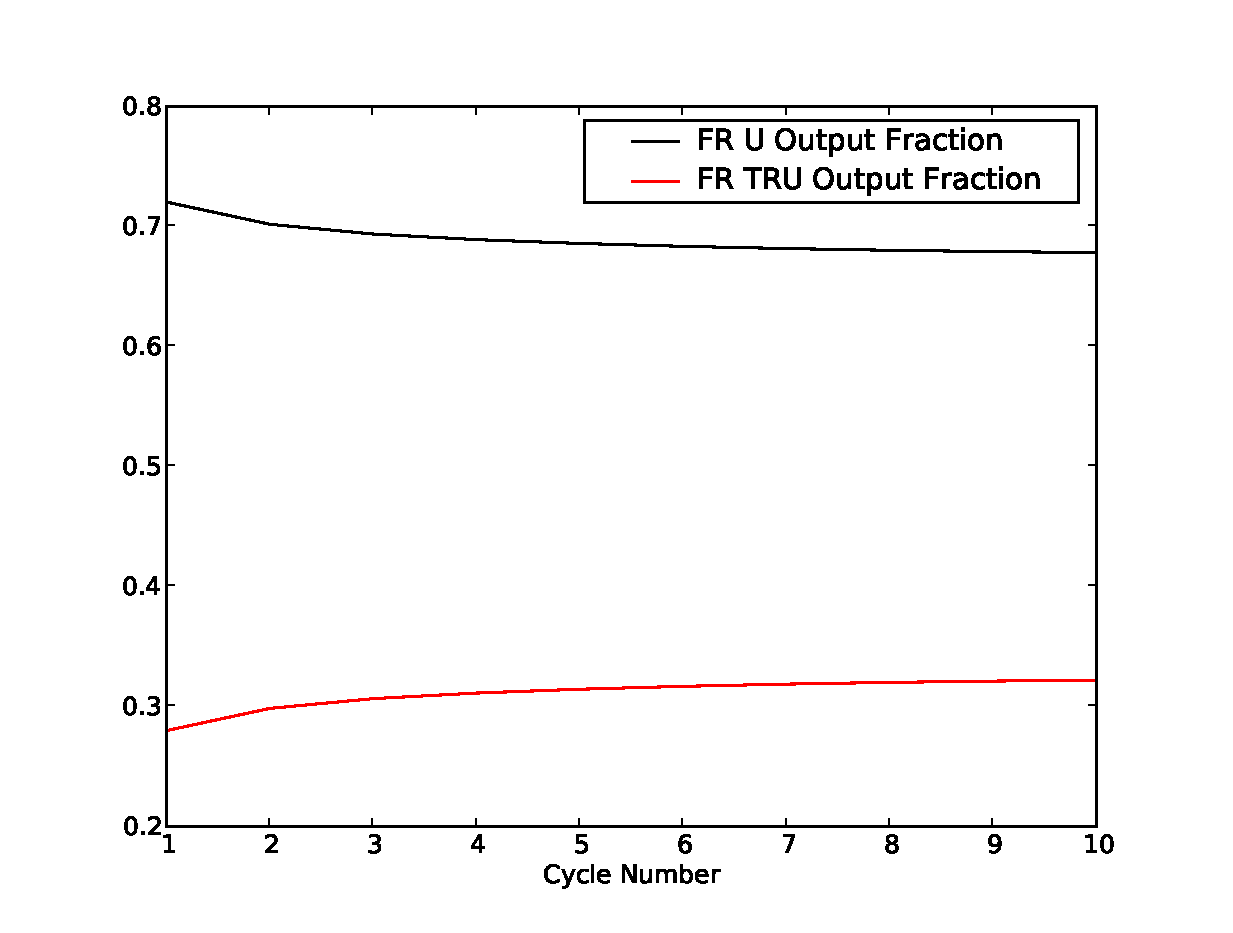
\includegraphics[scale=0.5]{se_sensitivity/figs/FRfracOut.eps}
\end{center}
\end{figure}

The transuranic conversion ratio (TRU CR) is defined as presented in the previous study.  
Here, TRU\subscript{in} is set as the sum of the LWR-TRU and FR-TRU stream mass
fractions as plotted in Figure \ref{ses_fig07}.  TRU\subscript{out} is the TRU 
mass fraction in the FR SNF stream.  Figure \ref{ses_fig09} shows that the TRU 
CR equilibrates at around 0.495.  Note that the CR is not an input to the model, but rather a
derived quantity that is a consequence of the reactor configuration and
discharge burnup.  The FR power fraction is likewise a derived quantity.
Figure \ref{ses_fig10} shows as a function of cycle number for the 99.9\% separation
efficiency case, the mass of LWR SNF needed to fabricate 1 kg of FR
fresh fuel.  For cycle numbers greater than 2, actinides from LWR fuel
serve as top-up only.  

\begin{figure}[htbp]
\caption{TRU Conversion Ratio}
\label{ses_fig09}
\begin{center}
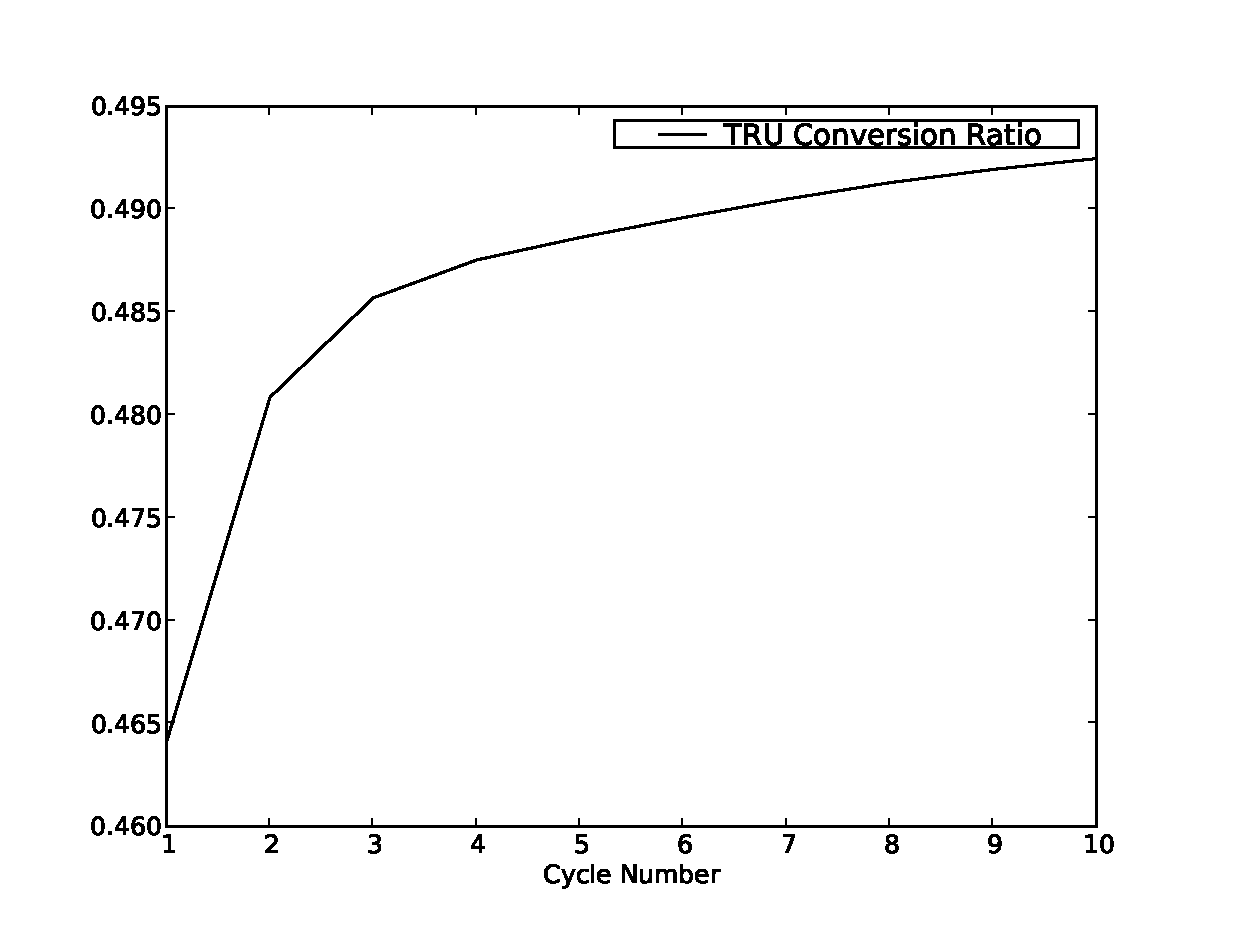
\includegraphics[scale=0.5]{se_sensitivity/figs/TruCR.eps}
\end{center}
\end{figure}

\begin{figure}[htbp]
\caption{LWR SNF Required to Top Up FR Fresh Fuel [kg LWR SNF/kg FR IHM]}
\label{ses_fig10}
\begin{center}
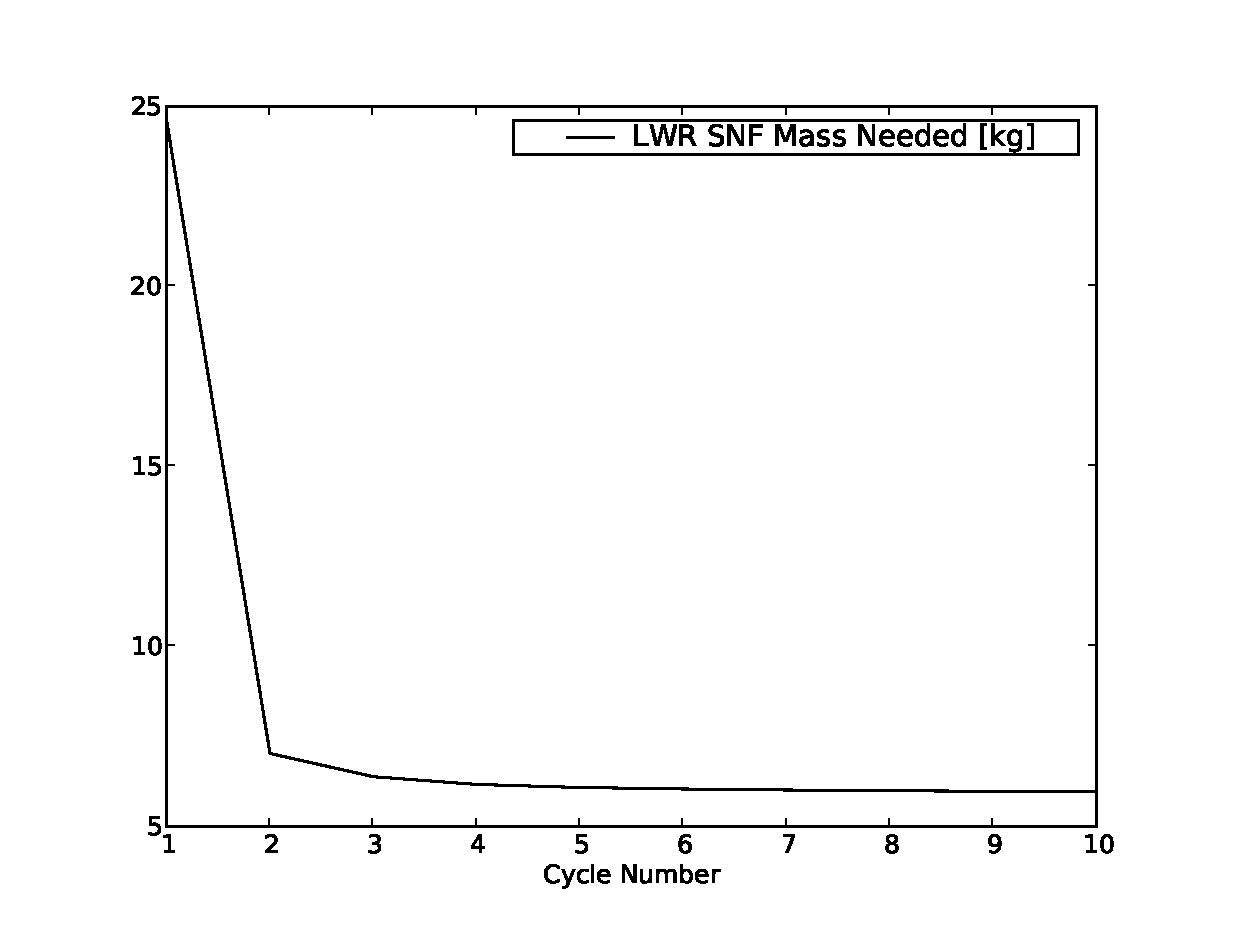
\includegraphics[scale=0.5]{se_sensitivity/figs/LWRsnfNeeded.eps}
\end{center}
\end{figure}


\subsubsection{Fuel Cycle Cost}
\index{Fuel Cycle Cost@\emph{Fuel Cycle Cost}}
\label{ses_sec:fcc}
Table \ref{ses_table12} shows the FCC computed according to the methods of Section 2.3
using the unit costs described in Section 3. For all strategies, higher
separation efficiencies (SE) lead to lower FCC while there is no
advantage for 99.99\% SE compared to 99.9\% SE.  Note that the
reprocessing cost is of necessity assumed to be independent of the
separation efficiency.  It is recognized that higher efficiencies will
require more separation stages and operation time, almost inevitably
leading to more costly plant operations.  However a review of literature
shows that the difficult task of correlating process costs to separation
efficiency has not yet been undertaken.

\begin{table}[htbp]
\begin{center}
\caption{FCC with Fixed Disposal Charge [\$/MWh]}
\label{ses_table12}
\begin{tabular}{|l|c|c|c|c|}
\hline
                & \textbf{Stra1} & \textbf{Stra2} & \textbf{Stra3} & \textbf{Stra4} \\
\hline
\textbf{Level1} & 5.51           & 5.51           & 5.50           & 5.50 \\
\textbf{Level2} & 5.18           & 5.18           & 5.16           & 5.16 \\
\textbf{Level3} & 5.15           & 5.14           & 5.13           & 5.12 \\
\textbf{Level4} & 5.14           & 5.14           & 5.13           & 5.12 \\
\hline
\end{tabular}
\end{center}
\end{table}



The FCC components are listed in detail in Tables \ref{ses_table13_0}-\ref{ses_table13_2}. At Level1, lower
separation efficiency results in more mass is reprocessed in the
reprocessing facility; hence the difference from the reprocessing charge
component dominates the small difference in FCC as one progresses to
more complex actinide partitioning strategies (Stra1 to Stra4).  When
the separation efficiency increases from 90\% to 99\% or 99.9\% the
annual charge for reprocessing service drops by around 10\%,
commensurate with the process mass reduction.  It is expected that the
unaccounted-for cost premium associated with achieving the higher
efficiencies would counteract this effect.  


\begin{table}[htbp]
\begin{center}
\caption{Cost Components for Cases 01-04}
\label{ses_table13_0}
\begin{tabular}{|l|c|c|c|c|}
\hline
\textbf{Components [\$/MWh]} & \textbf{case01} & \textbf{case02} & \textbf{case03} & \textbf{case04} \\
\hline
U Ore (yellow cake)          & 0.76            & 0.76            & 0.76            & 0.76 \\
U Conversion                 & 0.08            & 0.08            & 0.08            & 0.08 \\
U Enrichment                 & 1.11            & 1.11            & 1.11            & 1.11 \\
LWR Fuel Fabrication         & 0.44            & 0.44            & 0.44            & 0.44 \\
FR Fuel Fabrication          & 0.53            & 0.53            & 0.53            & 0.53 \\
Reprocessing                 & 1.93            & 1.93            & 1.93            & 1.93 \\
SNF Storage                  & 0.17            & 0.17            & 0.17            & 0.17 \\
LLW Disposal                 & 0.05            & 0.05            & 0.05            & 0.05 \\
LLW GTCC Disposal            & 0.00            & 0.00            & 0.00            & $<0.01$ \\
HLW/TRU Disposal             & 0.44            & 0.44            & 0.43            & 0.42 \\
\hline
\end{tabular}
\end{center}
\end{table}


\begin{table}[htbp]
\begin{center}
\caption{Cost Components for Cases 1-4}
\label{ses_table13_}
\begin{tabular}{|l|c|c|c|c|}
\hline
\textbf{Components [\$/MWh]} & \textbf{case1} & \textbf{case2} & \textbf{case3} & \textbf{case4} \\
\hline
U Ore (yellow cake)          & 0.69            & 0.69            & 0.69            & 0.69 \\
U Conversion                 & 0.07            & 0.07            & 0.07            & 0.07 \\
U Enrichment                 & 1.00            & 1.00            & 1.00            & 1.00 \\
LWR Fuel Fabrication         & 0.40            & 0.40            & 0.40            & 0.40 \\
FR Fuel Fabrication          & 0.67            & 0.67            & 0.67            & 0.67 \\
Reprocessing                 & 1.93            & 1.93            & 1.93            & 1.93 \\
SNF Storage                  & 0.16            & 0.16            & 0.16            & 0.16 \\
LLW Disposal                 & 0.05            & 0.05            & 0.05            & 0.05 \\
LLW GTCC Disposal            & 0.00            & 0.00            & 0.00            & $<0.01$ \\
HLW/TRU Disposal             & 0.21            & 0.21            & 0.19            & 0.18 \\
\hline
\end{tabular}
\end{center}
\end{table}


\begin{table}[htbp]
\begin{center}
\caption{Cost Components for Cases 11-14}
\label{ses_table13_1}
\begin{tabular}{|l|c|c|c|c|}
\hline
\textbf{Components [\$/MWh]} & \textbf{case11} & \textbf{case12} & \textbf{case13} & \textbf{case14} \\
\hline
U Ore (yellow cake)          & 0.68            & 0.68            & 0.68            & 0.68 \\
U Conversion                 & 0.07            & 0.07            & 0.07            & 0.07 \\
U Enrichment                 & 0.99            & 0.99            & 0.99            & 0.99 \\
LWR Fuel Fabrication         & 0.40            & 0.40            & 0.40            & 0.40 \\
FR Fuel Fabrication          & 0.69            & 0.69            & 0.69            & 0.69 \\
Reprocessing                 & 1.93            & 1.93            & 1.93            & 1.93 \\
SNF Storage                  & 0.16            & 0.16            & 0.16            & 0.16 \\
LLW Disposal                 & 0.05            & 0.05            & 0.05            & 0.05 \\
LLW GTCC Disposal            & 0.00            & 0.00            & 0.00            & $<0.01$ \\
HLW/TRU Disposal             & 0.19            & 0.18            & 0.17            & 0.16 \\
\hline
\end{tabular}
\end{center}
\end{table}


\begin{table}[htbp]
\begin{center}
\caption{Cost Components for Cases 21-24}
\label{ses_table13_2}
\begin{tabular}{|l|c|c|c|c|}
\hline
\textbf{Components [\$/MWh]} & \textbf{case21} & \textbf{case22} & \textbf{case23} & \textbf{case24} \\
\hline
U Ore (yellow cake)          & 0.68            & 0.68            & 0.68            & 0.68 \\
U Conversion                 & 0.07            & 0.07            & 0.07            & 0.07 \\
U Enrichment                 & 0.99            & 0.99            & 0.99            & 0.99 \\
LWR Fuel Fabrication         & 0.40            & 0.40            & 0.40            & 0.40 \\
FR Fuel Fabrication          & 0.69            & 0.69            & 0.69            & 0.69 \\
Reprocessing                 & 1.93            & 1.93            & 1.93            & 1.93 \\
SNF Storage                  & 0.16            & 0.16            & 0.16            & 0.16 \\
LLW Disposal                 & 0.05            & 0.05            & 0.05            & 0.05 \\
LLW GTCC Disposal            & 0.00            & 0.00            & 0.00            & $<0.01$ \\
HLW/TRU Disposal             & 0.19            & 0.18            & 0.17            & 0.16 \\
\hline
\end{tabular}
\end{center}
\end{table}



\subsubsection{Proliferation Resistance}
\index{Proliferation Resistance@\emph{Proliferation Resistance}}
\label{ses_sec:prilif_res}
The intrinsic proliferation resistance varies weakly between the cases
due to the separation efficiency and more strongly as a consequence of
partitioning strategy.  Table \ref{ses_table14} lists the system proliferation
resistance value for all cases.  Recall that higher numbers imply a
greater intrinsic proliferation resistance for the system.  Recall that
higher numbers imply a greater intrinsic proliferation resistance for
the system.  As an example, when applied to the OECD benchmark case
``scheme 1a'' (PWR-OT) this model generates a proliferation resistance
value of 0.2416.

The differences between cases arise from the reprocessing and HLW
disposal stages.  SNF storage and HLW disposal handle similar materials
and both represent pure storage sites.  Hence they share same level of
proliferation resistance. The large difference in inventory at HLW
disposal site as the partitioning strategy is varied generates
relatively large proliferation resistance differences at this stage.  FR
fuel fabrication, LWR reactor, FR reactor and reprocessing facility have
lower proliferation resistance value in the fuel cycle system due to the
large inventory of actinides Pu, Np, Am and Cm. Especially in the
reprocessing stage, the pure Pu in case01, case1 and case11 negatively
impact the proliferation resistance value.  The benefit of co-extraction
of Np, Am and Cm with Pu is shown to lead to the best proliferation
resistance value.

\begin{table}[htbp]
\begin{center}
\caption{System Proliferation Resistance Value}
\label{ses_table14}
\begin{tabular}{|l|c|c|c|c|}
\hline
                & \textbf{Stra1} & \textbf{Stra2} & \textbf{Stra3} & \textbf{Stra4} \\
\hline
\textbf{Level1} & 0.1850         & 0.1874         & 0.2421         & 0.2422 \\
\textbf{Level2} & 0.1853         & 0.1870         & 0.2418         & 0.2418 \\
\textbf{Level3} & 0.1852         & 0.1865         & 0.2414         & 0.2414 \\
\textbf{Level4} & 0.1852         & 0.1865         & 0.2413         & 0.2410 \\
\hline
\end{tabular}
\end{center}
\end{table}



\subsubsection{Repository Performance}
\index{Repository Performance@\emph{Repository Performance}}
\label{ses_sec:rep_perform}
The heat load based repository capacity is shown in Table \ref{ses_table15}.  The
benefit accrued by separating Am, Cm, Cs and Sr from the spent fuel is
considerable. At all three levels, by separating Am and Cm only, the
repository capacity doubles and further separation of Cs and Sr make the
repository capacity 3.7 times (level 1), 25.8 times (level 2), 228.5
times (level 3) and 1221.2 times (level 4) greater compared to strategy
1. 

\begin{table}[htbp]
\begin{center}
\caption{Repository Capacity [tIHM/Repository]}
\label{ses_table15}
\begin{tabular}{|l|c|c|c|c|}
\hline
                & \textbf{Stra1} & \textbf{Stra2} & \textbf{Stra3} & \textbf{Stra4} \\
\hline
\textbf{Level1} & 9342           & 9383           & 28766          & 34609 \\
\textbf{Level2} & 4849           & 4755           & 23341          & 124877 \\
\textbf{Level3} & 4388           & 4291           & 22555          & 1002783 \\
\textbf{Level4} & 4342           & 4244           & 22478          & 5302541 \\
\hline
\end{tabular}
\end{center}
\end{table}



The benefit of higher separation efficiency can be clearly appreciated
from the result in Table \ref{ses_table16} where the repository capacity is represented
as the total electricity generated from the HLW that may be placed in a
fully loaded repository. Higher separation efficiency leads to greater
economy of repository usage in all cases, but it is especially
noteworthy that only for Stra4, where Cs/Sr partitioning is pursued,
does it become worthwhile to achieve 99.99\% efficiency for all species.
 This result is simply a consequence of the capacity-limiting species
for each strategy.  In strategies 1 through 3, once 99.9\% efficiency is
reached, Cs and Sr become limiting, so that there is no further benefit
to reaching 99.99\% actinide separation efficiency unless Cs and Sr are
partitioned as well.  

\begin{table}[htbp]
\begin{center}
\caption{Repository Capacity [GWh/Repository]}
\label{ses_table16}
\begin{tabular}{|l|c|c|c|c|}
\hline
                & \textbf{Stra1} & \textbf{Stra2} & \textbf{Stra3} & \textbf{Stra4} \\
\hline
\textbf{Level1} & 2.96E+07       & 3.00E+07       & 9.39E+07       & 1.15E+08 \\
\textbf{Level2} & 3.26E+07       & 3.26E+07       & 1.71E+08       & 9.63E+08 \\
\textbf{Level3} & 3.30E+07       & 3.30E+07       & 1.86E+08       & 8.81E+09 \\
\textbf{Level4} & 3.30E+07       & 3.30E+07       & 1.88E+08       & 4.72E+10 \\
\hline
\end{tabular}
\end{center}
\end{table}




Note that the dramatic increase in the heat-based capacity of the
repository is not matched by commensurate decreases in HLW volume or
dose.  Table \ref{ses_table17} shows the mass of HLW generated by each unit of
electricity produced. Therefore, the capacity
enhancement shown in Table \ref{ses_table15} may not be accompanied by a proportionate
decrease in disposal cost; likewise, the potential dose of materials
placed in a fully loaded repository is many times higher for Stra4 than
for the other cases.  

\begin{table}[htbp]
\begin{center}
\caption{HLW Mass Per Unit Energy Produced [gHM/GWh]}
\label{ses_table17}
\begin{tabular}{|l|c|c|c|c|}
\hline
                & \textbf{Stra1} & \textbf{Stra2} & \textbf{Stra3} & \textbf{Stra4} \\
\hline
\textbf{Level1} & 315.5          & 312.9          & 306.4          & 300.0 \\
\textbf{Level2} & 148.8          & 145.8          & 136.9          & 129.7 \\
\textbf{Level3} & 133.2          & 130.2          & 121.0          & 113.8 \\
\textbf{Level4} & 131.6          & 128.7          & 119.5          & 112.2 \\
\hline
\end{tabular}
\end{center}
\end{table}




\section{Conclusions}
\index{Conclusions@\emph{Conclusions}}
\label{ses_sec:conclusions}
This paper has documented the development and benchmarking of a new
modeling framework that couples simple, physics-based models for fuel
cycle and reactor material balance generation, repository capacity, dose
and toxicity assessment, economics and proliferation resistance.  The
coupled model suite was created to investigate the sensitivity of these
important fuel cycle outcomes to changes in partitioning strategies and
elemental separation efficiency in reprocessing plants.

The modeling framework is unique because it links burnup and reactivity
calculations in which reactor performance and fuel cycle mass balance
are coupled with a fuzzy logic based barrier method for assessing
proliferation resistance, a repository thermal analysis tool and
multi-zonal transport model to treat repository performance and an
economic module.  The linkage is significant because perturbations to
system input variables such as separation efficiencies are propagated
through all the submodels: for instance, the material balance tool
recalculates the transient and equilibrium FR cycle material balances.

This new framework was applied to a GNEP-inspired LWR and transmuter 
FR fuel cycle architechture.  Partitioning strategies were varied with 
Np, Am/Cm, and Cs/Sr alternatively being partitioned for recycle or storage 
or sent to the repository with the low heat emitting fission products.
Elemental separation efficinecies were also varied with values of
90\% to 99.99\% being considered.  It was shown that the efficiency 
of repository space usage, meausred by the energy produced by the fuel from
which the HLW placed in the repository was derived, can ve imporved by 
more than two orders of magnitude if 99.99\% separation efficiency is 
achieved and Cs/Sr are partitioned.  If Cs/Sr are not partitioned, it was not seen
to be worthwhile to exceed 99.9\% efficiency.  On the other hand,
drastic increases in the low heat release fission product loading of the
repository may limit the potential repository benefit of the
transmutation scheme by increasing the dose, toxicity and mass to be
interred.

In the short term, it is of interest to consider the separation
efficiency for individual elements.  Perhaps capacity enhancement goals
can still be met even if 99.9\% or 99.99\% efficiency is not met at each
step - for example, if Cs/Sr efficiency is limited to 99.9\%, it
appears that achieving an equivalent TRU separation efficiency may not
be necessary; 99\% could suffice with the same repository benefit.  

In future, as understanding of the variation of disposal cost with
these parameters as well as the response of the reprocessing cost to
efficiency improves, system optimization will emerge as an important
area of study.  This self-contained, physics-based tool executes and
incorporates feedbacks between is components.  As such, a stochastic
system optimization wrapper that invokes the new tool could efficiently
search the parameter space.

Finally, only a single LWR/FR strategy has been considered thus far. 
Other fuel cycle strategies, for instance multi-tier approaches that
include partial transmutation in thermal systems, will also be
addressed.  Due to the presence of additional reprocessing steps, it is
expected that such strategies will respond even more sensitively to
variations in process efficiency.

